\documentclass[11pt, a4paper]{article}

\usepackage{graphicx}
\usepackage[a4paper,top=3cm,bottom=2cm,left=2cm,right=2cm,marginparwidth=1.75cm]{geometry}
\usepackage[english]{babel}
\usepackage[utf8x]{inputenc}
\usepackage{subfig}
\usepackage{float}
\usepackage{amsmath}
\usepackage{amssymb}
\usepackage{mhchem}
\usepackage{hyperref}
\usepackage{tikz}
\usepackage{cancel}

\graphicspath{ {./images} }
\newcommand*{\qed}{\hfill\ensuremath{\quad\square}}%
\newcommand*{\rad}{\ensuremath{\,\text{rad}}}
\newcommand*{\R}{\ensuremath{\mathbb{R}}}
\newcommand*{\C}{\ensuremath{\mathbb{C}}}
\renewcommand*{\Re}{\operatorname{Re}}
\renewcommand*{\Im}{\operatorname{Im}}
\renewcommand*{\epsilon}{\varepsilon}
\renewcommand*{\phi}{\varphi}

\makeatletter
\renewcommand*\env@matrix[1][*\c@MaxMatrixCols c]{%
  \hskip -\arraycolsep
  \let\@ifnextchar\new@ifnextchar
  \array{#1}}
\makeatother

\newtheorem{theorem}{Theorem}

%------------------------------------------------
%Templates for images and figures
% \begin{figure}[h]
%   \centering
%   \subfloat[caption 1]{{
\includegraphics[width=30mm]{images/placeholder.png}}}%
%   \qquad
%   \subfloat[caption 2]{{
\includegraphics[width=30mm]{images/placeholder.png}}}%
%   \caption{Description}
% \end{figure}

% \begin{figure}[h]
%   \centerline{
\includegraphics[width=50mm]{images/placeholder.png}}
%   \caption{Description}
% \end{figure}

%Template for a simple table 
%\begin{table}[h]
%   \caption{Description} %title of the table
%   \centering % centering table
%   \begin{tabular}{l rr} % creating three columns
%     \hline\hline %inserting double-line
%     & & \\ [0.5ex] % Insert half line vertical spacing
%     \hline % inserts single-line
%     & & \\ 
%     & & \\
%     & & \\
%     & & \\
%   \hline % inserts single-line
%   \end{tabular}
%   \label{tab:hresult}
% \end{table}
%-----------------------------------------------

\begin{document}
\setcounter{equation}{0}
\setcounter{section}{7}

\section{WOP3B Lecture 8: Static and dynamic loading of welds and rivits\footnote{Although the lecture mainly talks about welds it also applies the same to rivits} (04/06/2020)}


\subsection{Static loading on welds}
Recall the FBD of a weld:

\begin{figure}[H]
  \centerline{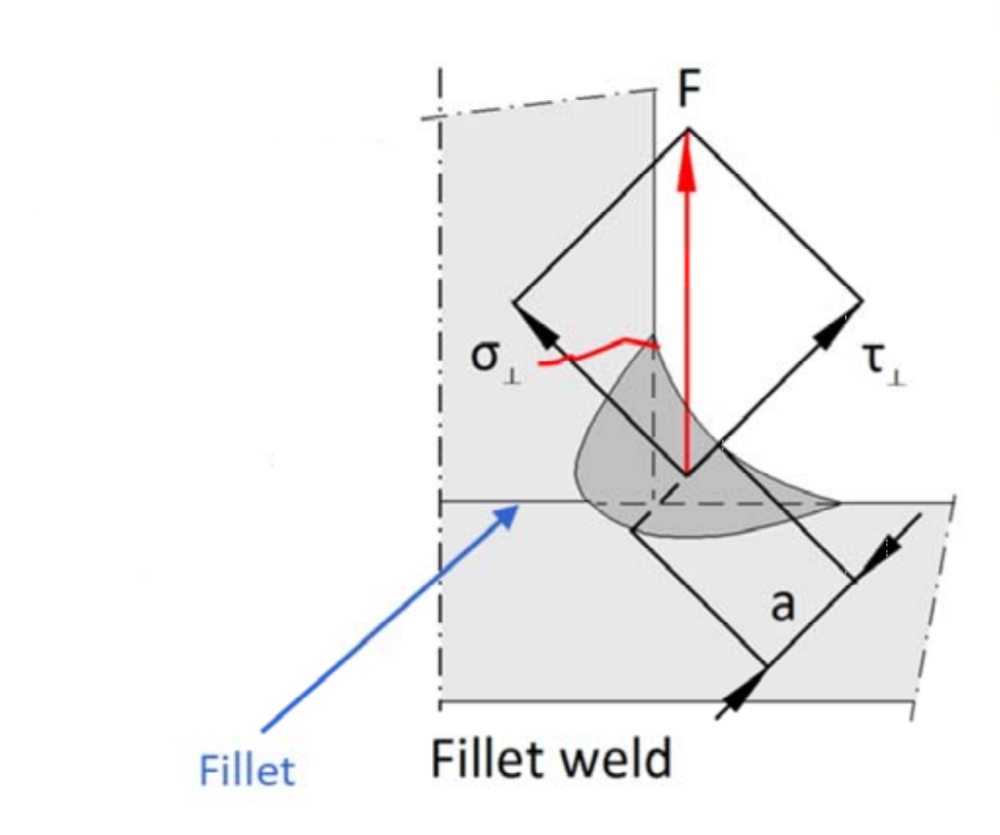
\includegraphics[width=80mm]{images/Fillet_weld.png}}
  \caption{The FBD of a typical fillet weld}
\end{figure}

The resulting force $F$ in a weld is made up of the 2 components $\sigma_\perp$ and $\tau_\perp$. Applying some mechanics of materials we find:

\begin{gather}
	\sigma_\perp = \tau_\perp = \frac{F/\sqrt{2}}{aL}\\
	\tau_\parallel = 0
\end{gather}

The equivalent stress is then given as:

\begin{equation}
	\sigma_{eq} = \frac{F\sqrt{2}}{aL}
\end{equation}

We usually do not consider stress concentrations for static loads on ductile materials. We saw before in the lecture on rotary bending fatigue this is a much more important factor under dynamic loads.



\subsection{Dynamic loads on welds}
As mentioned stress concentrations are very important to consider when analyzing dynamic loads. When looking at figure 1 we can see a small fillet between the welded parts. This fillet is a stress riser which decreases the endurance limit. Furthermore for static loads we only consider the weld depth $a$. The overall geometry of a weld is much more important to consider for dynamically loaded welds. Figure below shows some key difference is shapes of a weld.

\begin{figure}[H]
  \centerline{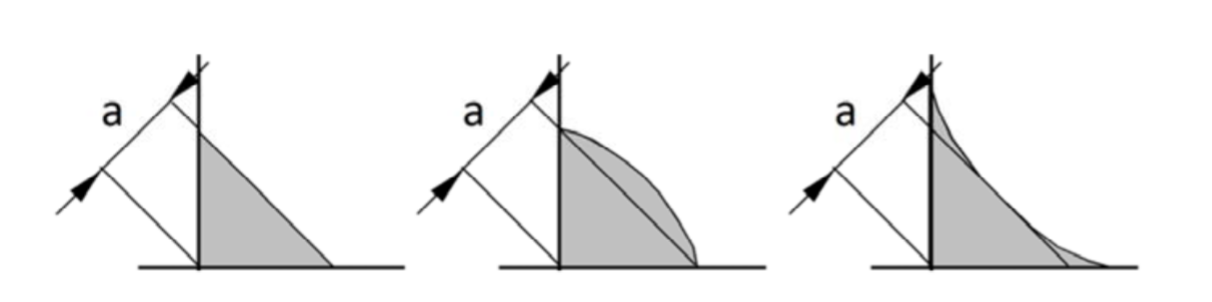
\includegraphics[width=120mm]{images/Weld_types.png}}
  \caption{Flat convex and concave welds where $a$ is the depth considered for static loading. The concave weld has a smoother transition in geometry and thus a lower local stress concentration.}
\end{figure}

Considering stress concentrations is especially important for butt-welds. The strength of butt welds does normally need to be considered as the strength of the weld will always be equal to or greater then the material that is being welded. When analyzing dynamic loads however the change in thickness will cause a local concentration in stress. Furthermore the local change in microstructure will make the material brittle and easier to fracture.

\begin{figure}[H]
  \centerline{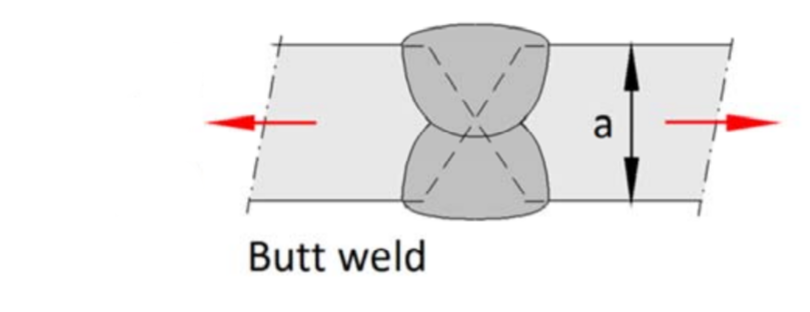
\includegraphics[width=100mm]{images/Butt_weld.png}}
  \caption{A typical butt-weld}
\end{figure}



\subsection{Detail categories of welds}
welds will via euronorm often be denoted with a detail category. The detail category is a standardized value for the endurance limit of a weld. The endurance limit of a weld will be given at $2(10)^6$ cycles. Because of this welds are almost always SLD rather then ILD. In figure 4 the general $SN$-curve for weld strength by category number is shown.

\begin{figure}[H]
  \centerline{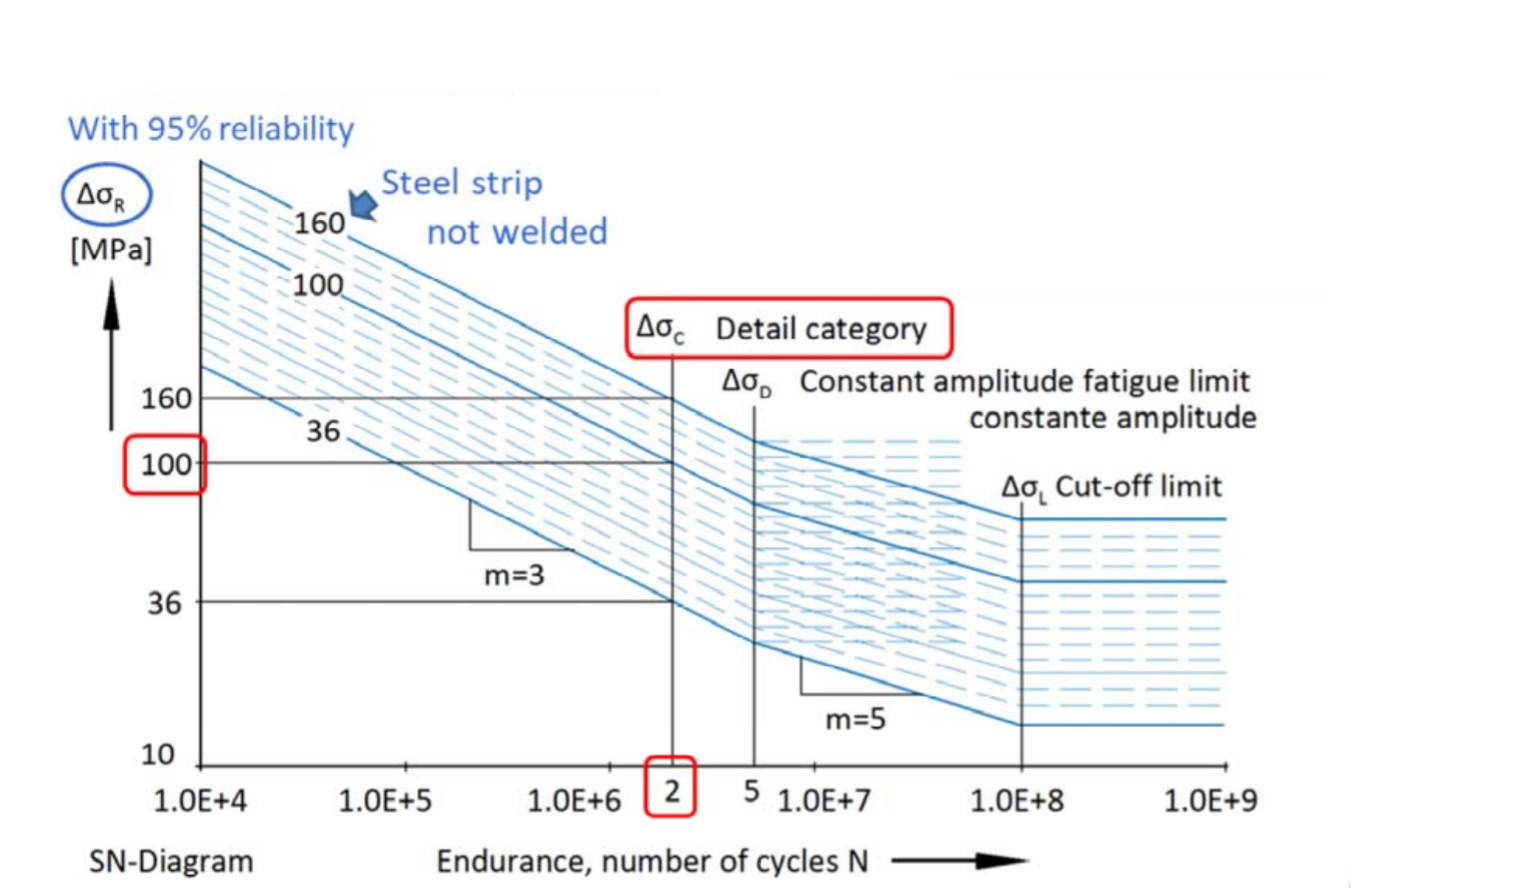
\includegraphics[width=120mm]{images/SN_curve.png}}
  \caption{The general $SN$-curve for the endurance limit. Category number of $160$ denotes an unwelded strip of steel.}
\end{figure}

\begin{gather}
	N_r = \left( \frac{\Delta \sigma_C}{\Delta \sigma_R} \right)^m N_C
	\begin{cases}
		m = 3, \sigma_R \geq \sigma_D\\
		m = 5, \sigma_D > \sigma_R \geq \Delta \sigma_C
	\end{cases}\\
	\Delta \sigma_D = \left( \frac{2}{5} \right)^{\frac{1}{3}} \Delta \sigma_C\\
	\Delta \sigma_C = \left( \frac{5}{100} \right)^{\frac{1}{5}} \Delta \sigma_D\\
\end{gather}

$N_R$ denotes the amount of cycles untill failure. $\sigma_C$ denotes the endurance limit based on the given weld category. $N_C = 2(10^6)$ and $\sigma_R$ is the applied load.



\subsection{High grade steel and welding}
Typically construction steel is used for welding. The high strength of an high grade ($>0.3\%$C) is usually reached through heat treatment. Welding steel will locally heat the steel changing the microstructure. This causes the strength of the joint to go back to that of a low carbon steel. Because of this applying higher grade steel is an ineffective and expensive solution.



\subsection{Methods of improving weld fatigue strength}
\begin{itemize}
	\item Omit welded joints
	\item Move welded joints to lower stress areas
	\item Select weld details with high detail category numbers
	\item Smooth geometric discontinuities
	\item Remedial surface grinding
	\item Post weld heat treatment
	\item Ultrasonic Impact Treatment (UIT), Hammer peening
\end{itemize}


\end{document}